% Build from this directory: lualatex -interaction=nonstopmode -halt-on-error main.tex
\documentclass[12pt,a4paper]{article}

\usepackage{fontspec,polyglossia}
\setdefaultlanguage{ukrainian}
\setmainfont{NewCM10-Regular.otf}[
  BoldFont=NewCM10-Bold.otf,
  ItalicFont=NewCM10-Italic.otf,
  BoldItalicFont=NewCM10-BoldItalic.otf
]
\setsansfont{Noto Sans}
\setmonofont{Noto Sans Mono}[Scale=0.82]

\usepackage{xurl}
\usepackage{geometry,graphicx,booktabs,array,enumitem,caption,titlesec,xcolor,fvextra,float}
\geometry{left=2cm,right=2cm,top=2cm,bottom=2cm}
\setlength{\parindent}{1.25cm}
\setlength{\parskip}{4pt}
\setlength{\emergencystretch}{3em}
\linespread{1.08}
\titleformat{\section}{\normalfont\fontsize{14}{16}\selectfont\bfseries}{\thesection}{0.6em}{}
\titleformat{\subsection}{\normalfont\fontsize{12}{14}\selectfont\bfseries}{\thesubsection}{0.6em}{}
\captionsetup{hypcap=false,font=small,labelfont=bf,labelsep=endash}
\DefineVerbatimEnvironment{code}{Verbatim}{fontsize=\footnotesize,breaklines=true,breakanywhere=true,frame=single,framesep=2mm}

\usepackage[
  unicode,
  colorlinks=true,
  linkcolor=black,
  urlcolor=blue,
  pdfauthor={Давидчук Артем},
  pdftitle={Архітектура комп'ютерів. Частина 2. Лабораторна робота №4}
]{hyperref}

\begin{document}

\pagenumbering{gobble}
\begin{titlepage}
  \begin{center}
    
\includegraphics[width=0.7\textwidth]{../../../../../../templates/letterhead.png}\\[1em]
    \large
    Національний технічний університет України\\
    «Київський політехнічний інститут імені Ігоря Сікорського»\\[1em]
    Факультет інформатики та обчислювальної техніки\\
    Кафедра обчислювальної техніки
  \end{center}

  \vfill
  \begin{center}
    \textbf{\LARGE Архітектура комп'ютерів}\\[0.4em]
    \textbf{\Large Частина 2. Процесори}\\[2em]
    \textbf{\Large Лабораторна робота №4}\\[0.7em]
    \parbox{0.9\textwidth}{\centering
      «Ядро Linux. Розроблення та перевірка завантажуваного модуля»}
  \end{center}

  \vfill
  \begin{flushright}
    Виконав: студент групи ІО-41\\
    \textit{Давидчук Артем}\\[1em]
    Перевірив: \textit{Каплунов А.~В.}
  \end{flushright}

  \vfill
  \begin{center}Київ --- 2026\end{center}
\end{titlepage}
\pagenumbering{arabic}

\section{Мета роботи}

Ознайомитися з технологією розроблення зовнішніх модулів ядра Linux,
системою збирання Kbuild, параметрами модулів, списками ядра, засобами
виділення пам'яті та вимірювання часу. Розробити, зібрати й перевірити модуль
для архітектури ARMv7 у середовищі QEMU.

\section{Постановка задачі}

За основу обрано другий із трьох наданих прикладів. Він використовує окремий
файл \texttt{Kbuild} для опису модуля та звичайний \texttt{Makefile} для
виклику системи збирання ядра.

Модуль повинен приймати параметр \texttt{count} типу \texttt{uint}, який
визначає кількість повідомлень \texttt{Hello, world!}. Значення за
замовчуванням дорівнює 1. Для значень 0 та від 5 до 10 модуль має вивести
попередження і продовжити роботу. Значення понад 10 має спричинити повернення
\texttt{-EINVAL} та відмову від завантаження.

Перед кожним привітанням потрібно виділити елемент списку, записати у нього
час \texttt{ktime\_get()} та додати до списку. Під час вивантаження модуля
необхідно надрукувати час усіх подій у наносекундах, вилучити елементи зі
списку та звільнити пам'ять.

Репозиторій із вихідним кодом і Makefile:
\begin{center}
\href{https://github.com/davidchyk/university_roadmap/tree/main/semester5/ca2/work/labs/lab4}{github.com/davidchyk/university\_roadmap/.../ca2/work/labs/lab4}
\end{center}

\section{Теоретичні відомості}

\subsection{Завантажуваний модуль ядра}

Завантажуваний модуль ядра є об'єктним файлом \texttt{.ko}, який можна
додати до працюючого ядра командою \texttt{insmod} і вилучити командою
\texttt{rmmod}. Функція, зареєстрована макросом \texttt{module\_init()},
викликається під час завантаження. Функція \texttt{module\_exit()}
викликається під час вивантаження.

На відміну від звичайної програми, модуль працює у просторі ядра. Він не має
функції \texttt{main()} та не використовує стандартну бібліотеку C.
Повідомлення записуються до журналу ядра функціями \texttt{pr\_info()},
\texttt{pr\_warn()} і \texttt{pr\_err()}, а переглядаються через
\texttt{dmesg}.

\subsection{Параметри, sysfs та modinfo}

Макрос \texttt{module\_param()} реєструє змінну як параметр модуля.
Права \texttt{0444} дозволяють читати встановлене значення у файловій
системі sysfs:

\begin{code}
cat /sys/module/hello/parameters/count
\end{code}

Макрос \texttt{MODULE\_PARM\_DESC()} додає текстовий опис, який відображає
команда \texttt{modinfo}. Поле \texttt{vermagic} у виводі \texttt{modinfo}
дає змогу перевірити сумісність модуля з версією та конфігурацією ядра.

\subsection{Список, пам'ять і час ядра}

Кожна подія представлена структурою з елементом \texttt{struct list\_head}
і часовою міткою \texttt{ktime\_t}. Макрос \texttt{LIST\_HEAD()} створює
порожню статичну голову двозв'язного списку. Нові елементи додаються через
\texttt{list\_add\_tail()}.

Пам'ять виділяється функцією \texttt{kmalloc()} з прапором
\texttt{GFP\_KERNEL}. Результат обов'язково перевіряється. Якщо виділення
не вдалося, функція ініціалізації повертає \texttt{-ENOMEM}, попередньо
звільнивши вже створені елементи. Безпечний обхід із вилученням виконується
макросом \texttt{list\_for\_each\_entry\_safe()}, після чого пам'ять
звільняється через \texttt{kfree()}.

Функція \texttt{ktime\_get()} повертає монотонний час ядра. Для виведення
значення в наносекундах використовується \texttt{ktime\_to\_ns()}.

\section{Програмна реалізація}

\subsection{Параметр і структура даних}

\begin{code}
struct hello_event {
    struct list_head list;
    ktime_t timestamp;
};

static unsigned int count = 1;
module_param(count, uint, 0444);
MODULE_PARM_DESC(count, "Number of times to print Hello, world!");

static LIST_HEAD(event_list);
\end{code}

\subsection{Ініціалізація модуля}

На початку перевіряється значення \texttt{count}. Для кожного привітання
створюється окремий елемент, у нього записується час, після чого елемент
додається до хвоста списку.

\begin{code}
if (count > 10) {
    pr_err("count=%u is greater than 10\n", count);
    return -EINVAL;
}

if (count == 0 || (count >= 5 && count <= 10))
    pr_warn("count=%u is unusual; continuing\n", count);

for (i = 0; i < count; i++) {
    event = kmalloc(sizeof(*event), GFP_KERNEL);
    if (!event) {
        free_events(false);
        return -ENOMEM;
    }

    event->timestamp = ktime_get();
    list_add_tail(&event->list, &event_list);
    pr_info("Hello, world!\n");
}
\end{code}

\subsection{Вивантаження та очищення}

Допоміжна функція обходить список, за потреби друкує часові мітки, вилучає
кожен елемент і звільняє його пам'ять. Ця сама функція забезпечує коректне
очищення у випадку частково виконаної ініціалізації.

\begin{code}
list_for_each_entry_safe(event, next, &event_list, list) {
    if (print_timestamps)
        pr_info("event time: %lld ns\n",
                (long long)ktime_to_ns(event->timestamp));

    list_del(&event->list);
    kfree(event);
}
\end{code}

Повний текст реалізації наведено у додатку А.

\section{Збирання і перевірка стилю}

Для роботи використано вже зібране ядро Linux 4.19.325 з ЛР №3 та
кроскомпілятор GNU Arm Toolchain 8.3-2019.03.

\begin{code}
export KDIR="$HOME/bbb-lab/repos/linux-stable"
export ARCH=arm
export CROSS_COMPILE="ccache arm-eabi-"
export PATH="$HOME/bbb-lab/toolchains/\
gcc-arm-8.3-2019.03-x86_64-arm-eabi/bin:$PATH"
\end{code}

Файл \texttt{Kbuild} містить одну ціль:

\begin{code}
obj-m := hello.o
\end{code}

Зовнішній \texttt{Makefile} передає каталог модуля до Kbuild:

\begin{code}
KDIR ?= /lib/modules/$(shell uname -r)/build

all:
    $(MAKE) -C $(KDIR) M=$(CURDIR) modules

clean:
    $(MAKE) -C $(KDIR) M=$(CURDIR) clean
\end{code}

Перед збиранням виконано перевірку стилю:

\begin{code}
$KDIR/scripts/checkpatch.pl --no-tree -f hello.c
\end{code}

Отримано результат \texttt{0 errors, 0 warnings}. Команда \texttt{file}
визначила \texttt{hello.ko} як 32-бітний ARM EABI5 relocatable ELF.
Значення \texttt{vermagic} дорівнює
\texttt{4.19.325 SMP mod\_unload ARMv7 p2v8}, тобто відповідає ядру QEMU.

\begin{figure}[H]
  \centering
  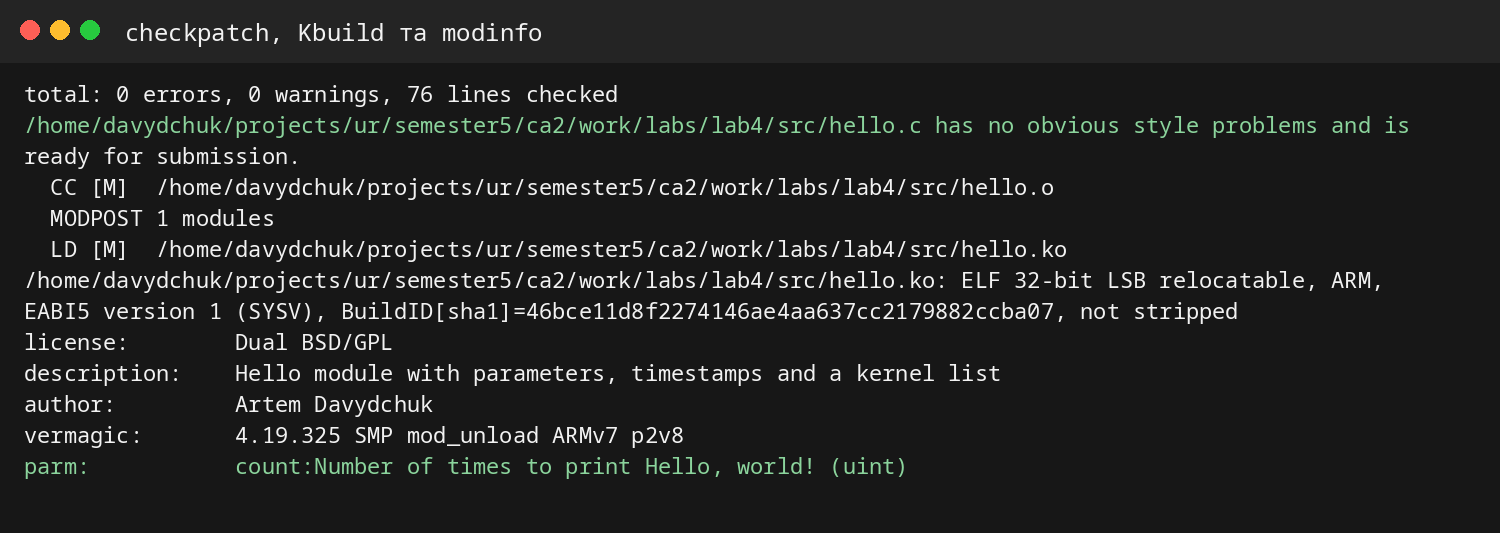
\includegraphics[width=\textwidth]{media/build-checkpatch-modinfo.png}
  \caption{Перевірка стилю, збирання модуля та команда modinfo}
\end{figure}

\section{Підготовка QEMU}

До окремої копії initramfs із ЛР №3 додано файл
\texttt{/root/hello.ko}. Початковий архів не змінювався. Тестова система
запускалася таким чином:

\begin{code}
qemu-system-arm \
  -machine virt -m 512 -nographic \
  -kernel "$HOME/bbb-lab/repos/busybox/_install/boot/zImage" \
  -initrd build/initramfs/rootfs-lab4.cpio.gz \
  -append "root=/dev/ram0 rw console=ttyAMA0,115200 mem=512M"
\end{code}

Ядро повідомило версію \texttt{4.19.325} та архітектуру
\texttt{armv7l}. Повідомлення про \texttt{out-of-tree module taints kernel}
є очікуваним: ядро фіксує завантаження зовнішнього модуля, якого немає в
основному дереві вихідних кодів.

\section{Результати перевірки}

Виконано п'ять сценаріїв. Перед кожним сценарієм журнал очищувався командою
\texttt{dmesg -c}, щоб результати не змішувалися.

\begin{table}[H]
\centering
\small
\begin{tabular}{c p{0.31\textwidth} p{0.41\textwidth}}
\toprule
\textbf{count} & \textbf{Результат insmod} & \textbf{Спостереження}\\
\midrule
не задано & модуль завантажено & одне привітання; параметр у sysfs дорівнює 1; під час rmmod надруковано один час\\
0 & модуль завантажено & попередження; привітання відсутні; параметр дорівнює 0\\
3 & модуль завантажено & три привітання і три часові мітки; параметр дорівнює 3\\
7 & модуль завантажено & попередження; сім привітань і сім часових міток; параметр дорівнює 7\\
11 & відмова, код 1 у shell & повідомлення про помилку; \texttt{-EINVAL}; модуль відсутній у lsmod\\
\bottomrule
\end{tabular}
\caption{Результати тестування параметра count}
\end{table}

\begin{figure}[H]
  \centering
  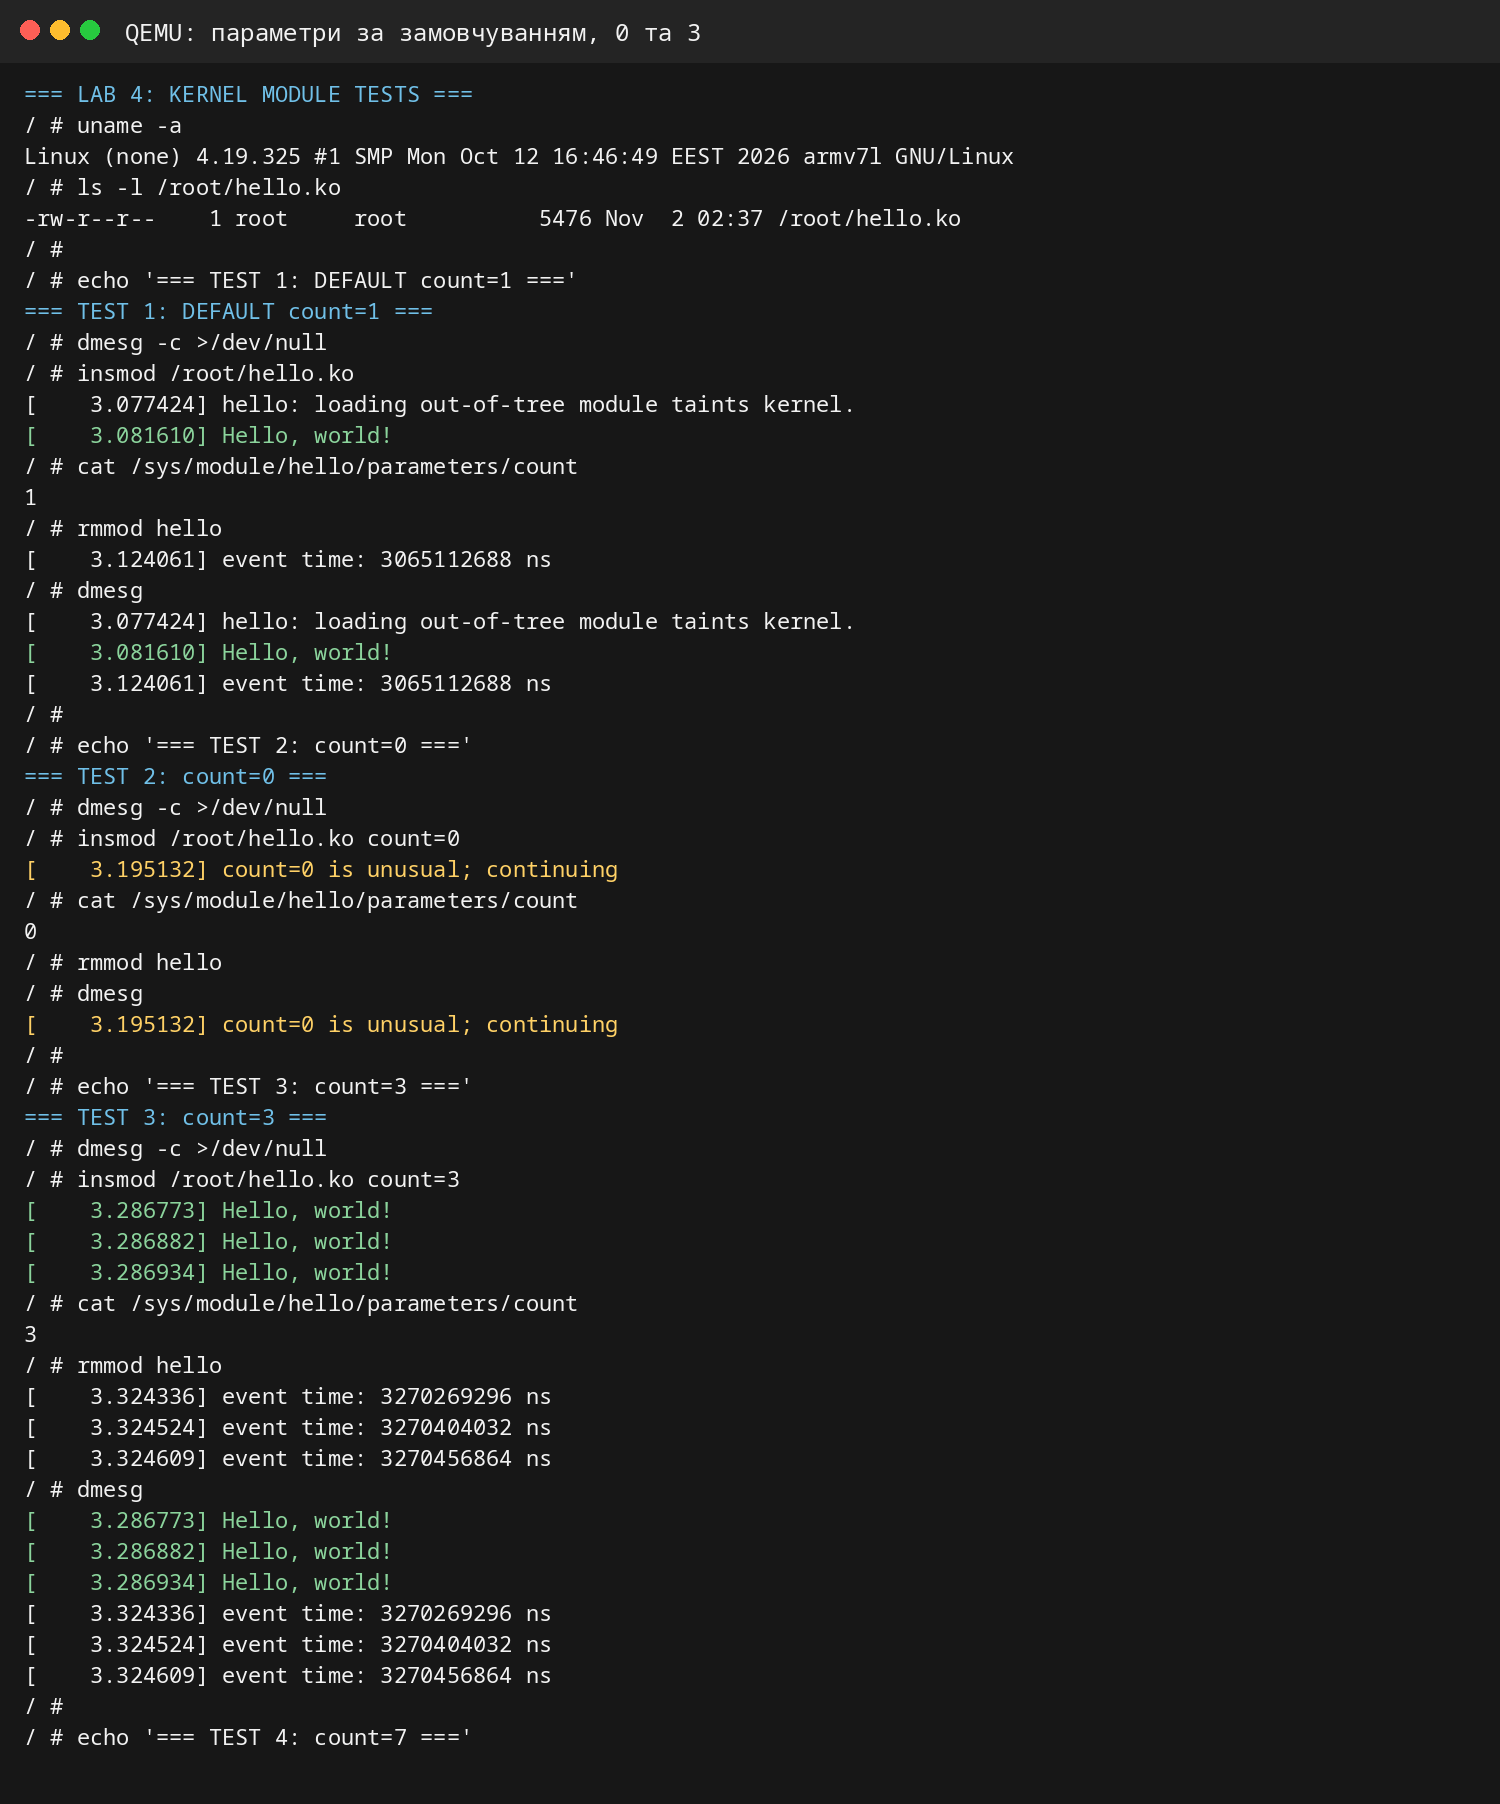
\includegraphics[width=0.68\textwidth]{media/qemu-tests-1-3.png}
  \caption{Перевірка значень за замовчуванням, 0 і 3 у QEMU}
\end{figure}

\begin{figure}[H]
  \centering
  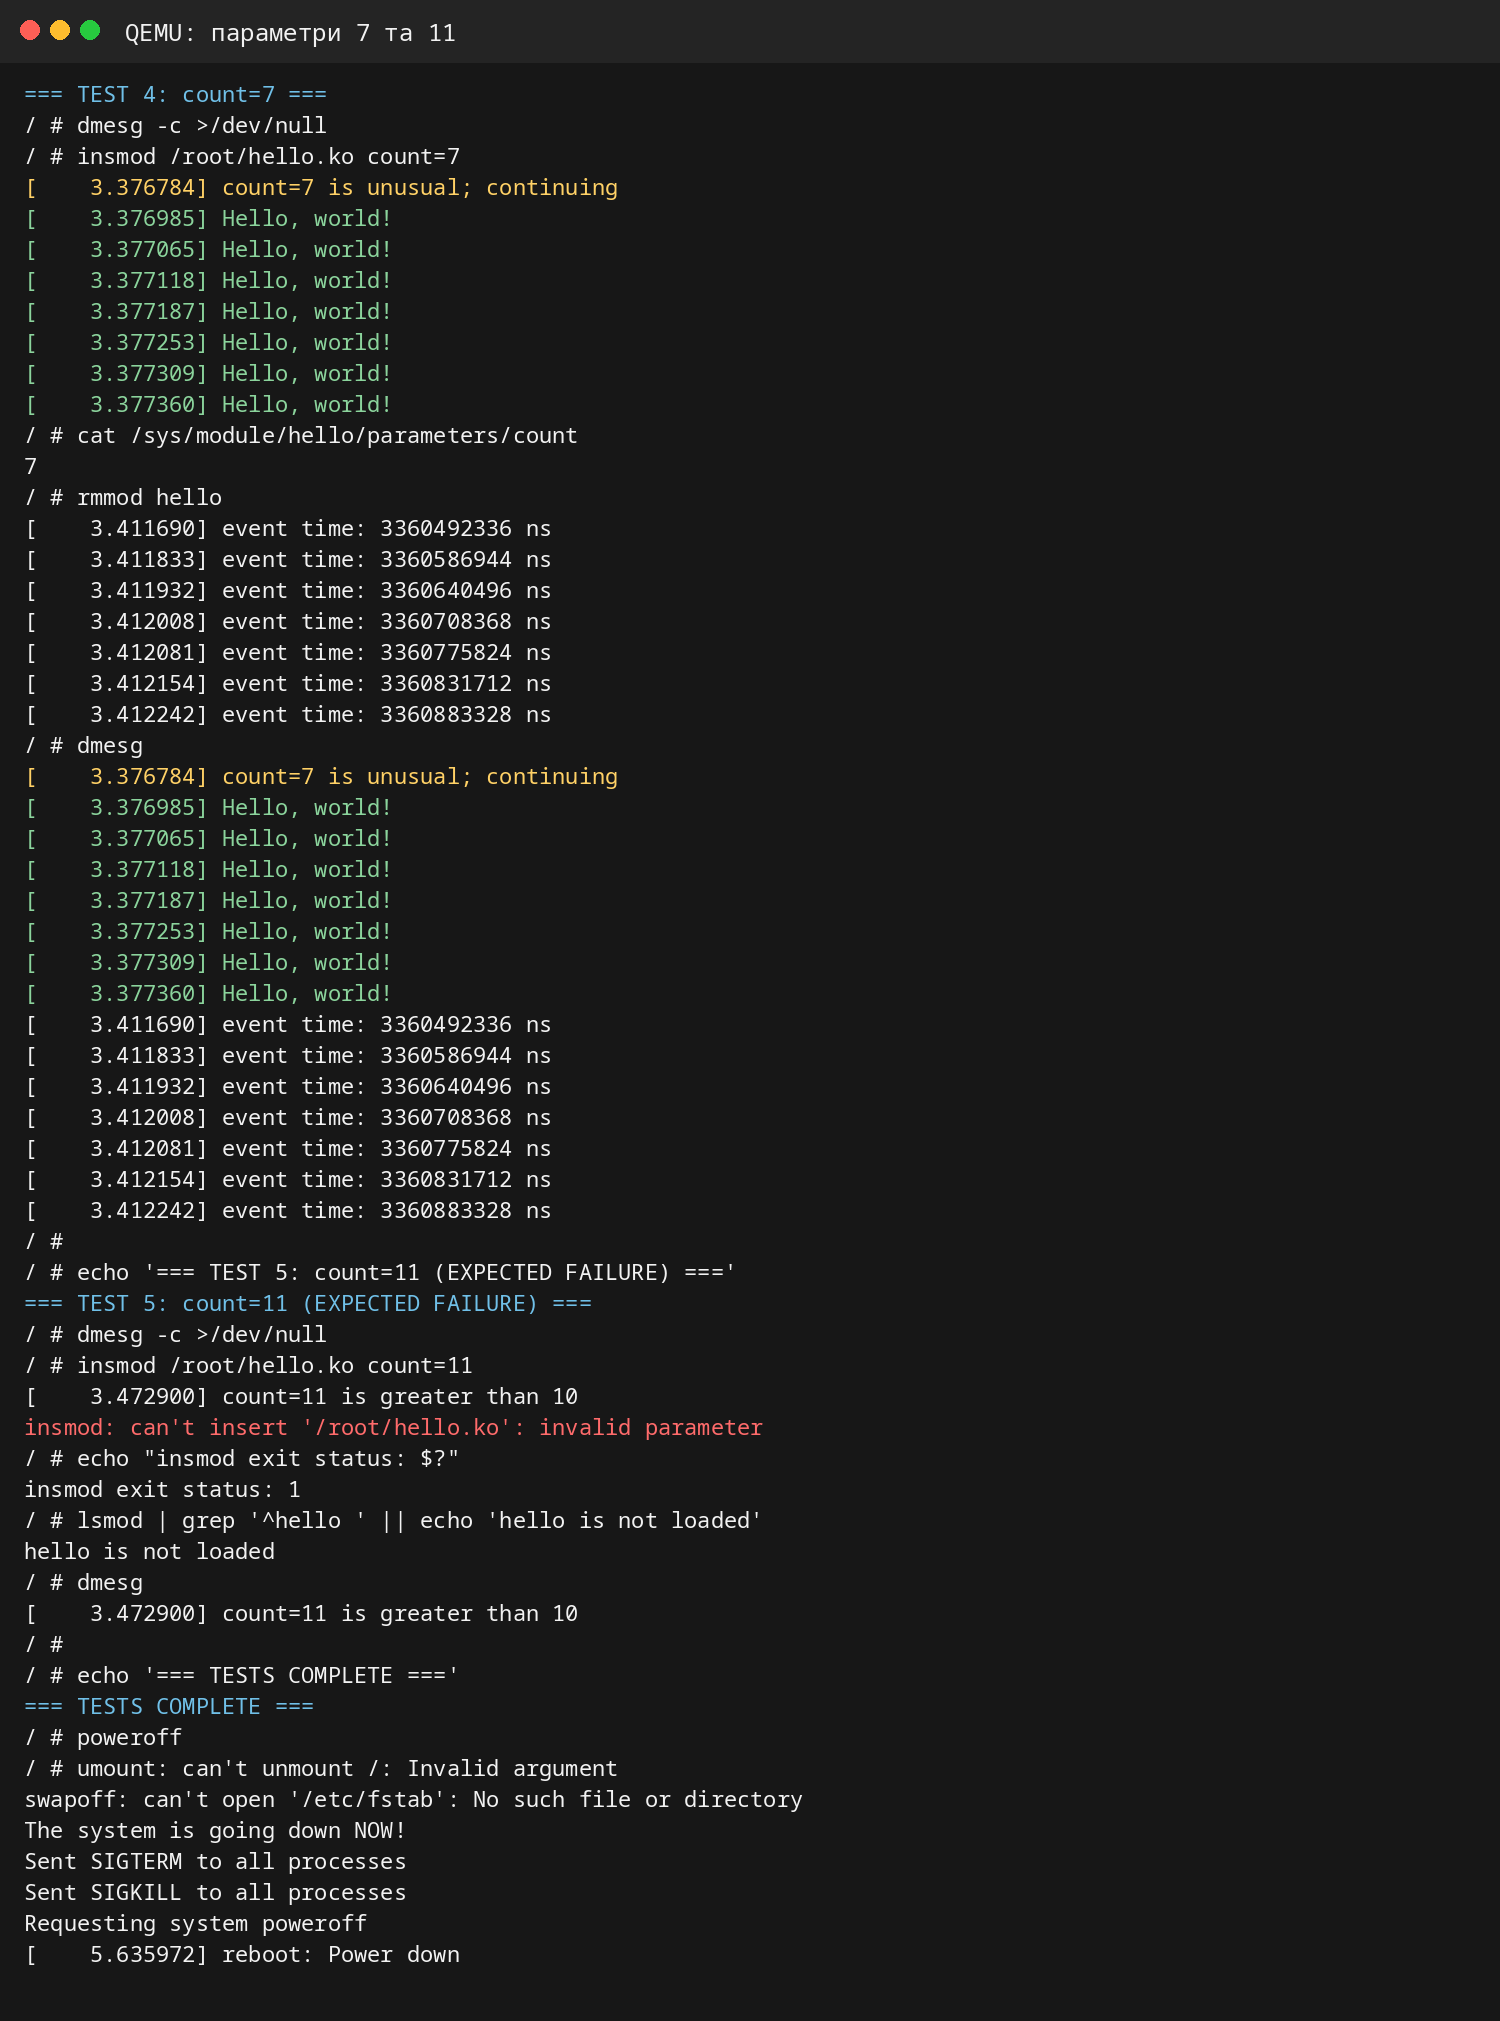
\includegraphics[width=0.62\textwidth]{media/qemu-tests-4-5.png}
  \caption{Перевірка значень 7 і 11 у QEMU}
\end{figure}

Значення встановленого параметра читалося після успішного \texttt{insmod}
з файла \path{/sys/module/hello/parameters/count}. Для \texttt{count=11}
команда \texttt{insmod} завершилася зі статусом 1, а перевірка
\texttt{lsmod} підтвердила, що модуль не завантажено.

Під час \texttt{rmmod} для кожного створеного елемента надруковано окрему
часову мітку в наносекундах. Кількість часових міток збіглася з кількістю
привітань, що підтверджує коректне додавання елементів до списку та їхній
обхід під час очищення.

Повний вивід збережено у форматах TXT і HTML у каталозі
\texttt{evidence}.

\section{Висновки}

У лабораторній роботі розроблено зовнішній модуль ядра Linux для ARMv7.
Модуль приймає параметр типу \texttt{uint}, перевіряє його допустимість,
створює задану кількість подій і зберігає їхні часові мітки у двозв'язному
списку ядра. Під час вивантаження часові мітки виводяться, елементи
вилучаються зі списку, а пам'ять звільняється.

Модуль успішно пройшов \texttt{checkpatch.pl} без помилок і попереджень,
був зібраний для Linux 4.19.325 та перевірений у QEMU. Тестування підтвердило
правильну поведінку для значень 0, 1, 3, 7 і 11, роботу параметра через
sysfs, відображення опису в \texttt{modinfo} та відмову від завантаження з
кодом \texttt{-EINVAL} для значення понад 10.

\section*{Використані матеріали}

\begin{enumerate}[leftmargin=*]
  \item Методичні вказівки до лабораторної роботи №4 «Виконання завдання щодо збирання модулів ядра».
  \item Приклади \texttt{test1}, \texttt{test2}, \texttt{test3} із наданого архіву \texttt{examples.zip}.
  \item Документація ядра Linux: \path{Documentation/kbuild/modules.txt}
    та \path{Documentation/process/coding-style.rst}.
  \item Вихідний код Linux 4.19.325 та результати виконання ЛР №3.
\end{enumerate}

\newpage
\section*{Додаток А. Повний текст hello.c}
\addcontentsline{toc}{section}{Додаток А. Повний текст hello.c}

\VerbatimInput[
  fontsize=\tiny,
  breaklines=true,
  breakanywhere=true,
  frame=single,
  framesep=2mm
]{../src/hello.c}

\end{document}
